\documentclass[10pt, aspectratio=169]{beamer}

\setbeamertemplate{frametitle}[default][center]
\setbeamertemplate{navigation symbols}{}
\setbeamertemplate{footline}[frame number]


\title{Journal Club}
\author{Valentin Marteau}
\date{31.05.2022}

\begin{document}

\frame{\titlepage}

\begin{frame}{Paper}
\centering
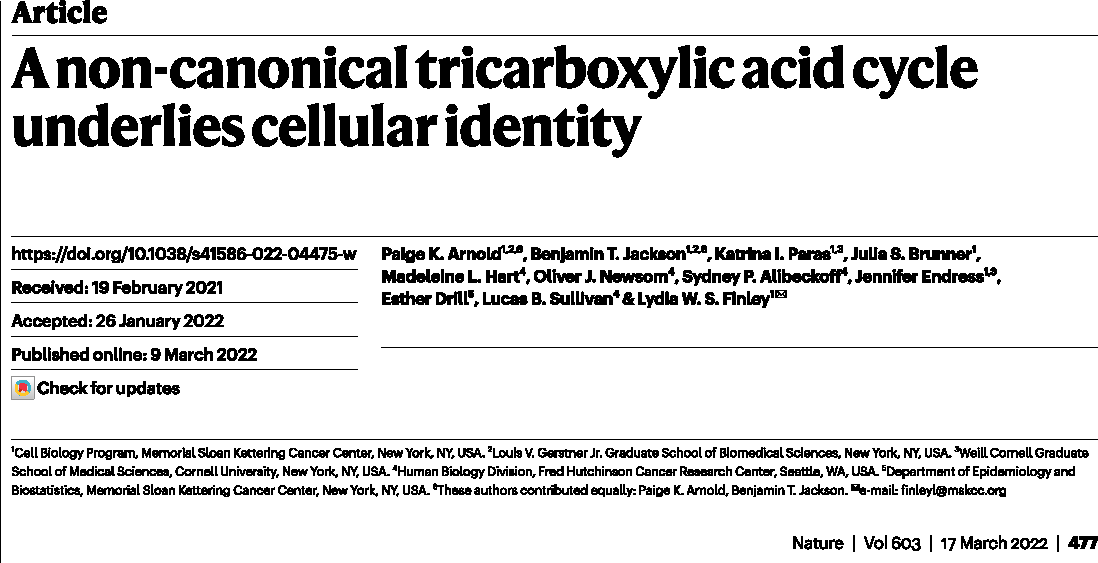
\includegraphics[width=0.9\textwidth]{figures/Arnold_2022_title.pdf}
\end{frame}


\begin{frame}{Aim}

Tricarboxylic acid (TCA) cycle: 

mammalian cells display diversity in TCA-cycle activity

How is this diversity achieved?
Is the TCA cycle critical for establishing cell fate?

\end{frame}

\begin{frame}{DepMap project}

\end{frame}

\begin{frame}{Two modes of TCA-cycle metabolism}

\end{frame}

\begin{frame}{ES cells engage a non-canonical TCA cycle}

\end{frame}

\begin{frame}{TCA-cycle choice is cell-state dependent}

\end{frame}

\begin{frame}{TCA-cycle switch after pluripotency exit}

\end{frame}

\begin{frame}{Exit from pluripotency requires ACL}

\end{frame}

\begin{frame}{Summary}

\end{frame}

\begin{frame}{Questions to be addressed}

\end{frame}

\begin{frame}{Take home messages}

Include Otto Warburg Grant Proposal?
\end{frame}

\end{document}





